\section{Design FPU}

Ta có thiết kế tổng quan của bộ tính toán FPU:

\begin{figure}[H]
	\centering
	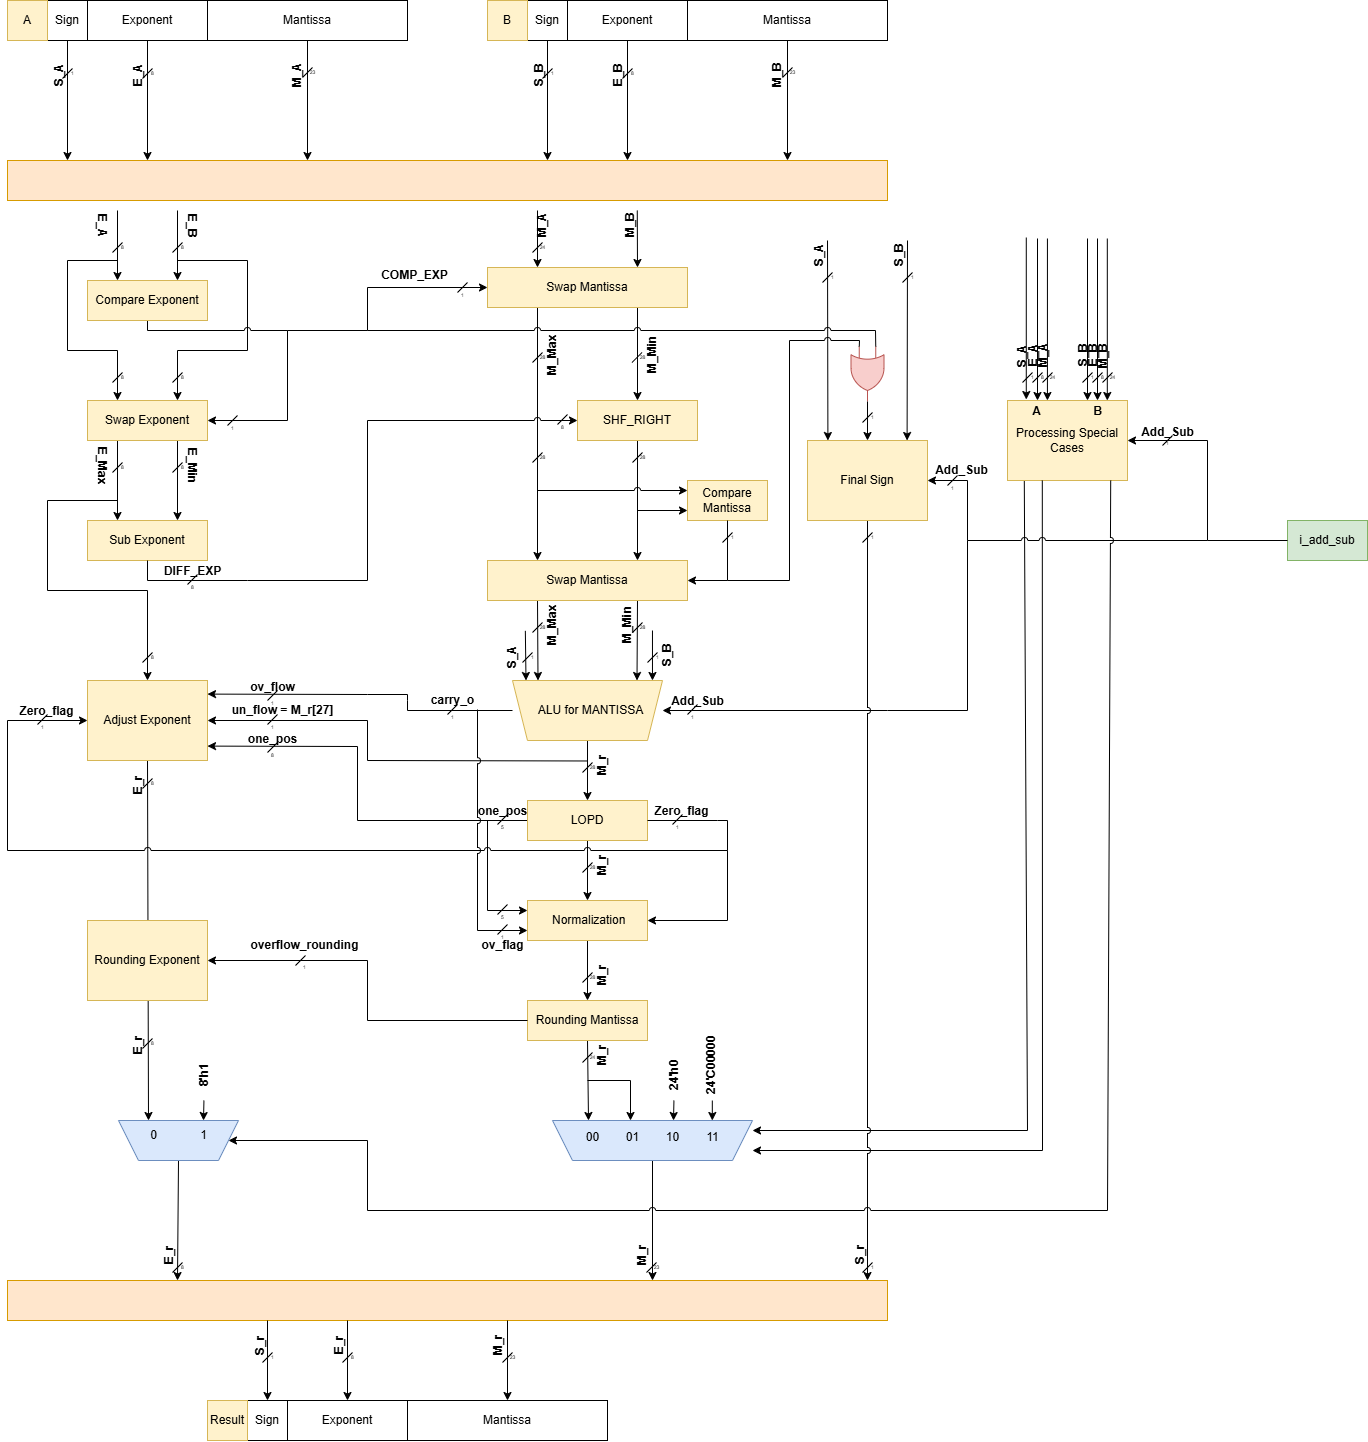
\includegraphics[width=.9\linewidth]{./my-chapters/my-diagrams/BlockDiagram_Overview.png}
	\caption{Sơ đồ khổi tổng quan của bộ FPU.}
\end{figure}

\subsection{Bộ tiền xử lý liên quan đến Exponent}

\begin{figure}[H]
	\centering
	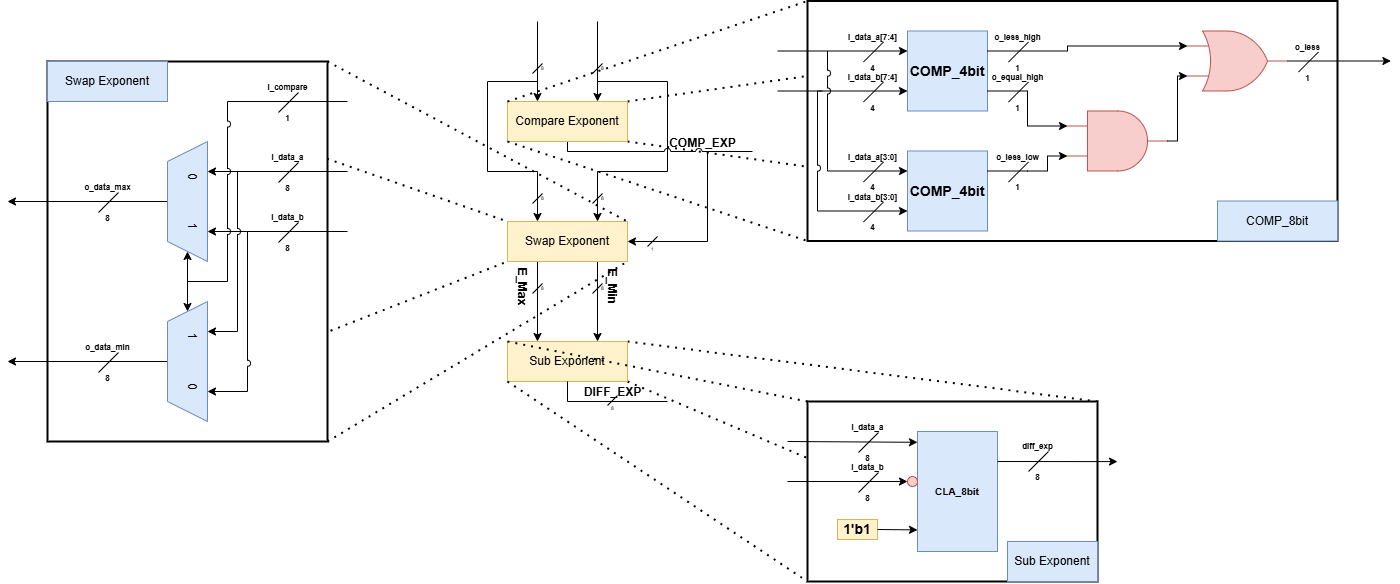
\includegraphics[width=\linewidth]{./my-chapters/my-diagrams/Exponent_Block_1.png}
	\caption{Bộ tính toán giá trị $| \text{EXP\_A} - \text{EXP\_B} |$.}
\end{figure}

Bộ có chức năng thực hiện tính giá trị trị khác nhau giữa hai Exponent của A và B.  Trong đó,

\begin{itemize}[label=-]
	\item Bộ \textsf{COMP\_4bit}: là bộ so sánh 4-bit hai số được triển khai dựa vào bảng sự thật và rút gọn bìa K như sau:
	
	\begin{minipage}{.45\linewidth}
		\begin{figure}[H]
			\centering
			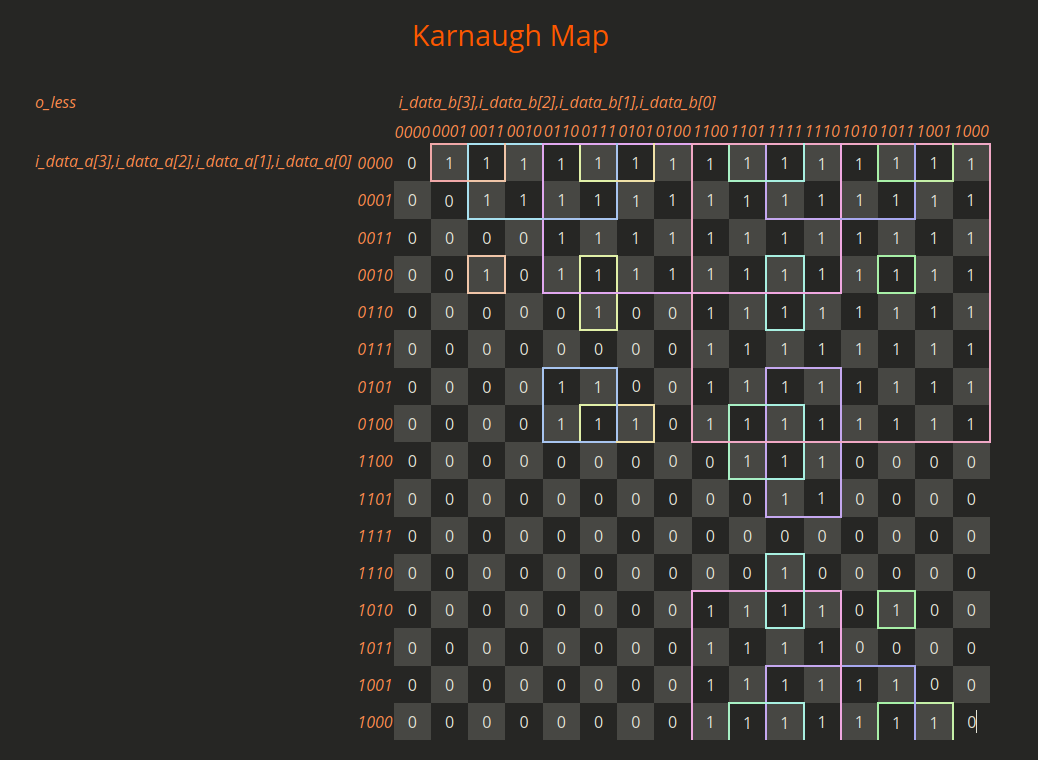
\includegraphics[width=\linewidth]{./my-chapters/my-images/K_maps/comp_4bit.png}
			\caption{Bìa K của bộ so sánh 4-bit (\textsf{COMP\_4bit}).}
		\end{figure}
	\end{minipage}
	\hspace{0.5cm}
	\begin{minipage}{.45\linewidth}
%		 \begin{table}[h] % or [t], [b], [!ht], etc.
%			 \centering
%			 \begin{tabular}{|>{\centering\arraybackslash}m{.5cm}
%			                 |>{\centering\arraybackslash}m{.5cm}
%			                 |>{\centering\arraybackslash}m{.5cm}
%			                 |>{\centering\arraybackslash}m{.5cm}
%			                 |>{\centering\arraybackslash}m{.5cm}
%			                 |>{\centering\arraybackslash}m{.5cm}
%			                 |>{\centering\arraybackslash}m{.5cm}
%			                 |>{\centering\arraybackslash}m{.5cm}
%			                 |>{\centering\arraybackslash}m{.5cm}|}
%		     \hline
%		     \multirow{4}{*}{\textsf{i\_data\_a}} & \multirow{4}{*}{\textsf{i\_data\_b}} & \multicolumn{2}{c|}{\textsf{COMP\_LESS}} \\
%		     
%			 \end{tabular}
%			 \caption{Bảng sự thật của \textsf{COMP\_4bit}.}
%	 	\end{table}
		\begin{lstlisting}[style=StyleCode, language=SystemVerilog, caption={Rút gọn từ Bìa K của bộ so sánh 4-bit (\textsf{COMP\_4bit}).}]
			assign o_less = (~i_data_a[3] & ~i_data_a[2] & ~i_data_a[1] & ~i_data_a[0] & i_data_b[0]) | (~i_data_a[3] & ~i_data_a[2] & ~i_data_a[1] & i_data_b[1]) | (~i_data_a[3] & ~i_data_a[2] & i_data_b[2]) | (~i_data_a[3] & i_data_b[3]) | (~i_data_a[3] & ~i_data_a[2] & ~i_data_a[0] & i_data_b[1] & i_data_b[0]) | (~i_data_a[3] & ~i_data_a[1] & ~i_data_a[0] & i_data_b[2] & i_data_b[0]) | (~i_data_a[3] & ~i_data_a[1] & i_data_b[2] & i_data_b[1]) | (~i_data_a[3] & ~i_data_a[0] & i_data_b[2] & i_data_b[1] & i_data_b[0]) | (~i_data_a[2] & ~i_data_a[1] & ~i_data_a[0] & i_data_b[3] & i_data_b[0]) | (~i_data_a[2] & ~i_data_a[1] & i_data_b[3] & i_data_b[1]) | (~i_data_a[2] & i_data_b[3] & i_data_b[2]) | (~i_data_a[2] & ~i_data_a[0] & i_data_b[3] & i_data_b[1] & i_data_b[0]) | (~i_data_a[1] & ~i_data_a[0] & i_data_b[3] & i_data_b[2] & i_data_b[0]) | (~i_data_a[1] & i_data_b[3] & i_data_b[2] & i_data_b[1]) | (~i_data_a[0] & i_data_b[3] & i_data_b[2] & i_data_b[1] & i_data_b[0]);
			
			assign o_equal = ~|(i_data_a ^ i_data_b);
		\end{lstlisting}
	\end{minipage}
\end{itemize}

\subsection{Bộ tiền xử lý liên quan đến Mantissa}

\begin{figure}[H]
	\centering
	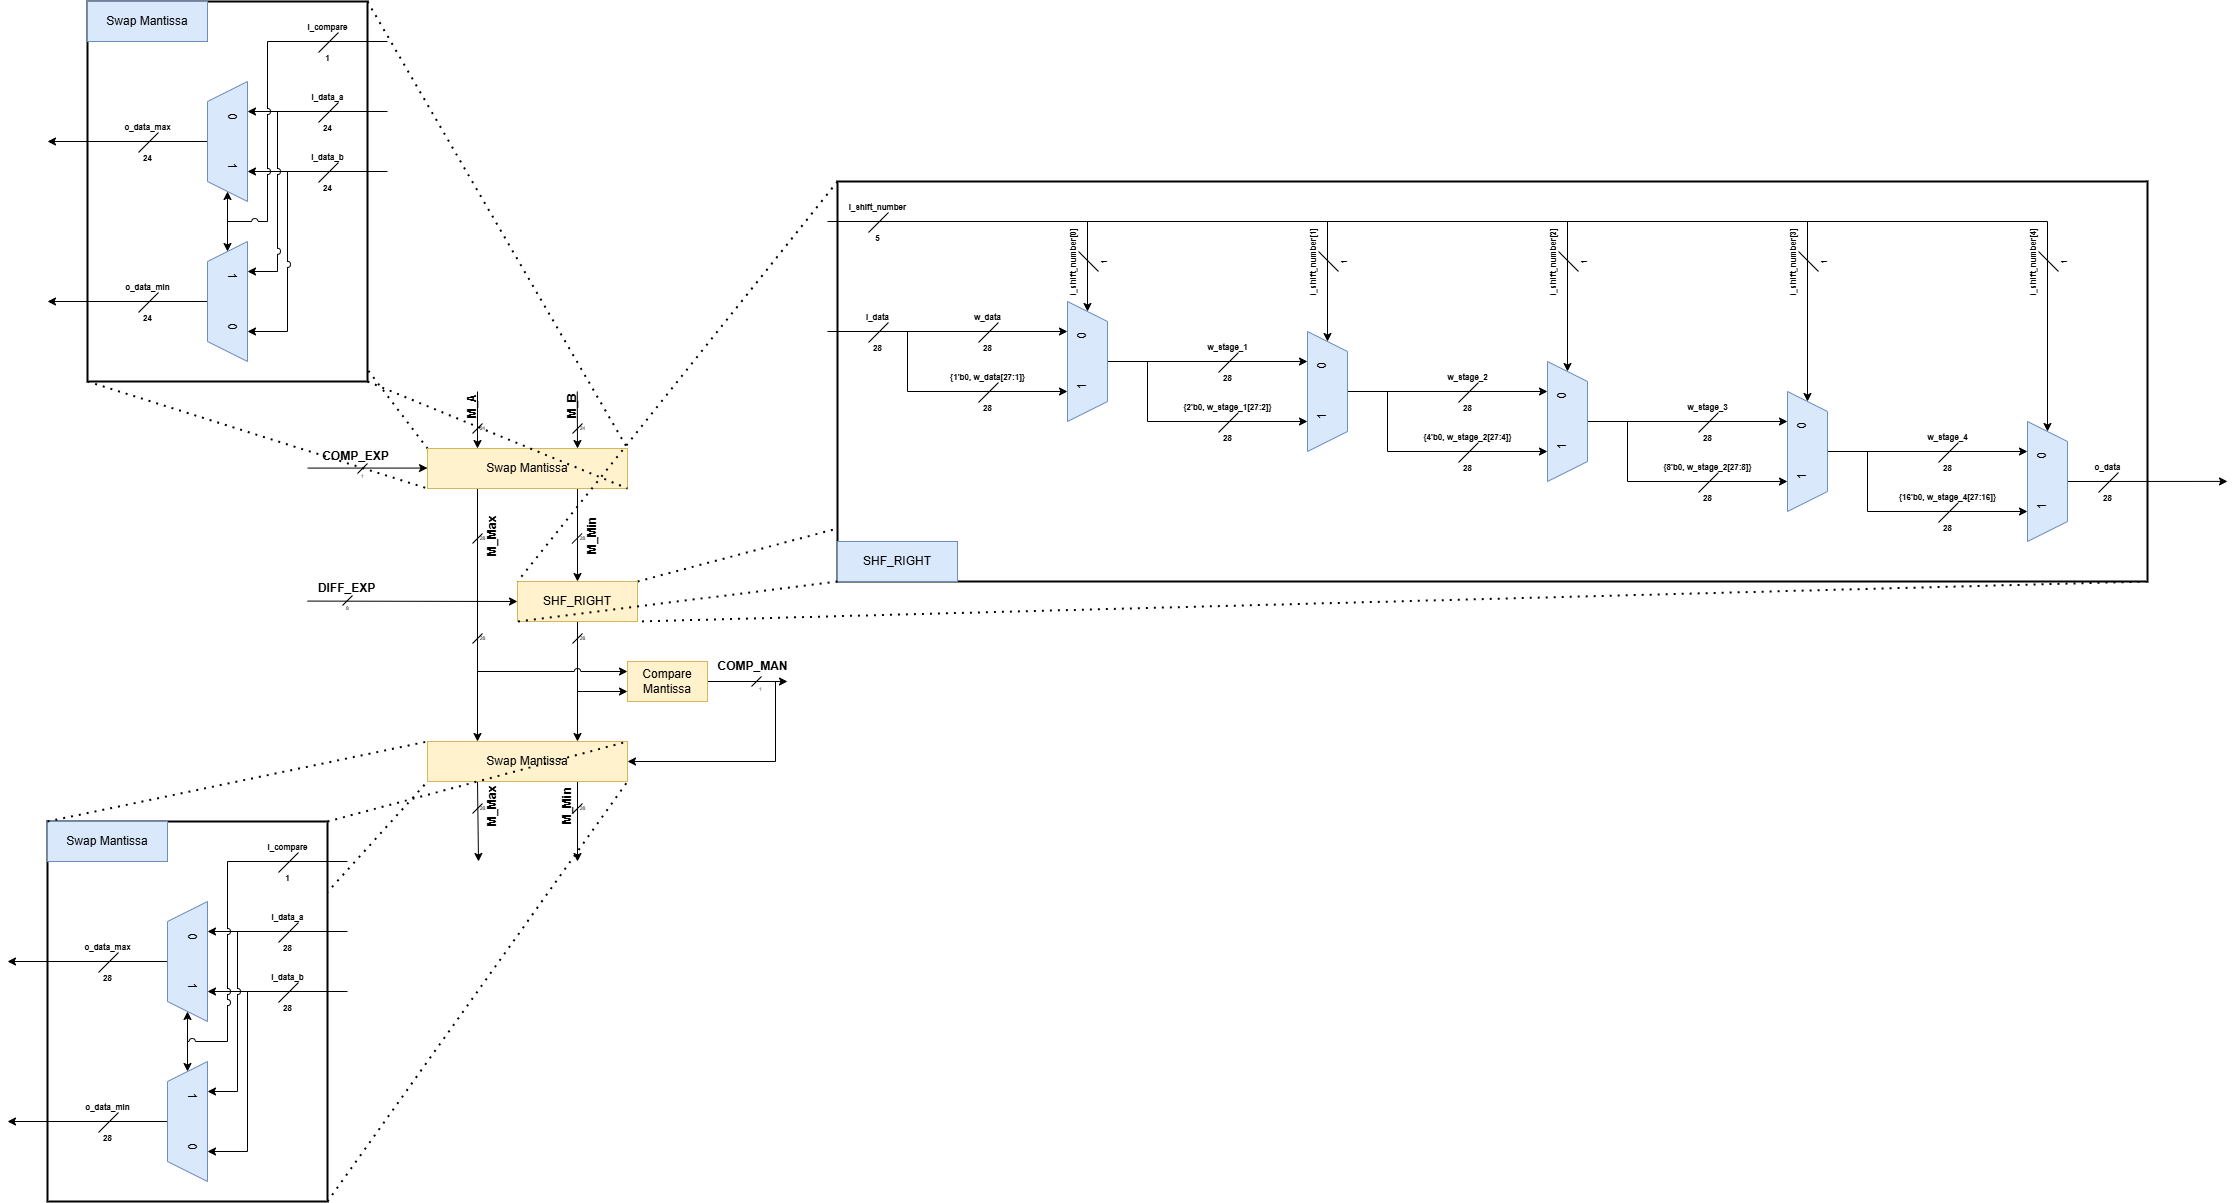
\includegraphics[width=\linewidth]{./my-chapters/my-diagrams/man_swap.png}
\end{figure}

Bộ Compare Mantissa, nhóm em đề xuất hai phương pháp như sau:

\begin{enumerate}[label=Phương pháp \arabic*., leftmargin=2cm]
	\item Sử dụng phương pháp xây dựng từ bộ \textsf{COMP\_4bit} để tạo nên bộ \textsf{COMP\_28bit} như sau:
		\begin{figure}[H]
			\centering
			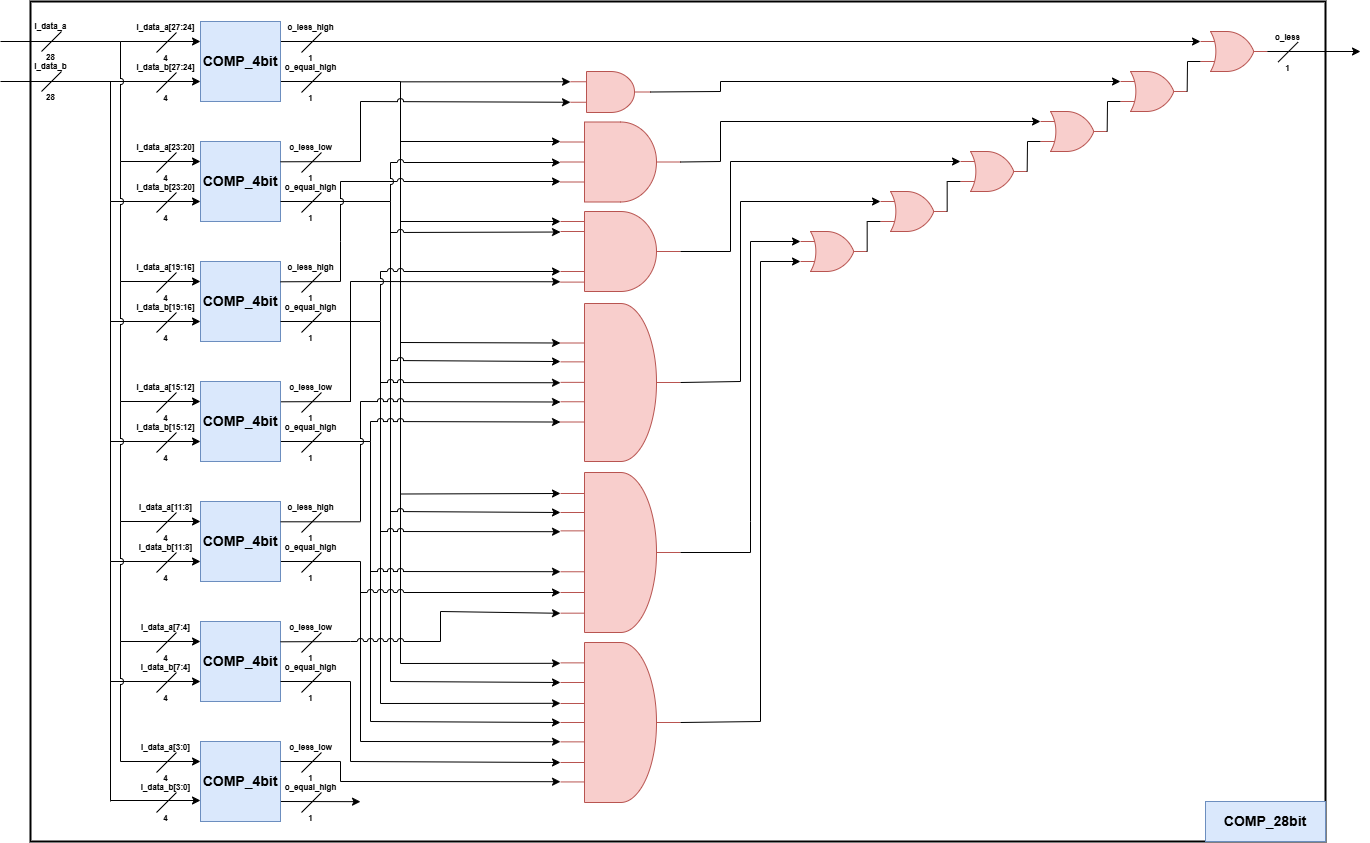
\includegraphics[width=.9\linewidth]{./my-chapters/my-diagrams/comp_28bit.png}
			\caption{Bộ so sánh 28-bit sử dụng các so sánh lan truyền.}
			\label{fig: comp_28bit_using_propagation_lessandequal}
		\end{figure}
	\item Sử dụng giải thuật cộng của bộ CLA (Carry Lookahead Adder) như sau:
		\begin{figure}[H]
			\centering
			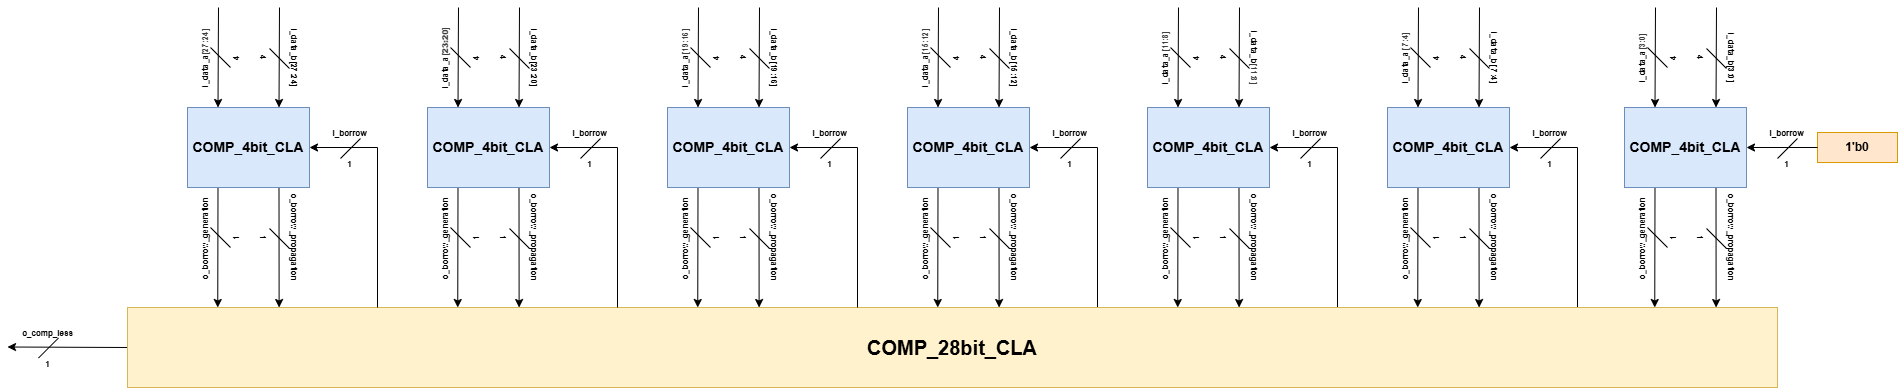
\includegraphics[width=.9\linewidth]{./my-chapters/my-diagrams/COM_28bit_1.png}
			\caption{Bộ so sánh 28-bit sử dụng phép trừ sử dụng giải thuật của bộ CLA.}
		\end{figure}
		
		Tuy nhiên với bộ tạo ra tín hiệu \texttt{P} và \texttt{G} sẽ khác do đây là phép trừ hai bit được biểu dưới dạng như:
		
		\begin{figure}[H]
			\centering
			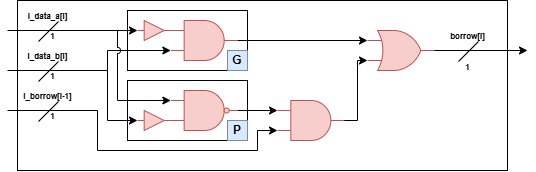
\includegraphics[width=.9\linewidth]{./my-chapters/my-diagrams/COM_28bit_1_unit.png}
		\end{figure}
		
		Và từ đó sẽ tiền hành như bộ CLA.
\end{enumerate}

Từ hai phương pháp trên, nhóm em quyết định sử dụng bộ \ref{fig: comp_28bit_using_propagation_lessandequal} để có thể dễ dàng triển khai bộ \texttt{COMP\_28bit}.

\subsection{Bộ xử lý dấu của phép tính}

\begin{figure}[H]
	\centering
	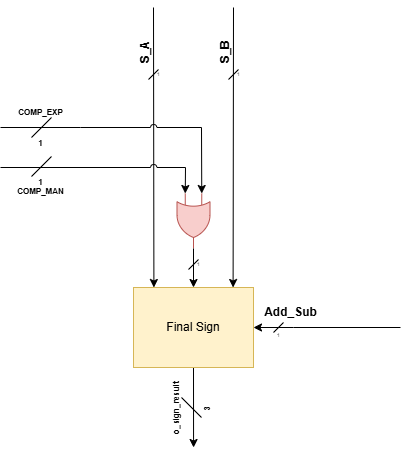
\includegraphics[width=.5\linewidth]{./my-chapters/my-diagrams/Final_sign.png}
\end{figure}

\begin{table}[H] % or [t], [b], [!ht], etc.
	\centering
	\begin{tabular}{|>{\centering\arraybackslash}m{2cm}
			|>{\centering\arraybackslash}m{2cm}
			|>{\centering\arraybackslash}m{2cm}
			|>{\centering\arraybackslash}m{2cm}
			|>{\centering\arraybackslash}m{2.5cm}
			|>{\raggedright\arraybackslash}m{5cm}|}
		\hline
		\textsf{i\_add\_sub} 	& \textsf{i\_sign\_a}	& \textsf{i\_sign\_b}	& \textsf{i\_comp}	& \textsf{o\_sign\_result} 	& \\
		\hline
		0	& 0	& 0	& X	& 0	& $(A + B) > 0$ \\
		\hline
		0	& 0	& 1 & 0 & 0 & $(A \geq B) \rightarrow (A - B) > 0$	\\
		\hline
		0 	& 0 & 1 & 1 & 1 & $(A < B) \rightarrow (A - B) < 0$ \\
		\hline
		0	& 1 & 0 & 0 & 1 & $(A \geq B) \rightarrow (- A + B) < 0$ \\
		\hline
		0	& 1 & 0 & 1 & 0 & $(A < B) \rightarrow (-A + B) > 0$\\
		\hline
		0 	& 1	& 1 & X & 1 & $(-A - B) < 0$ \\
		\hline
		1	& 0	& 0 & 0	& 0 & $(A \geq B) \rightarrow (A - B) > 0$ \\
		\hline
		1	& 0	& 0 & 1 & 1	& $(A < B) \rightarrow (A - B) < 0$ \\
		\hline
		1	& 0	& 1 & X & 0	& $(A - -B) > 0$ \\
		\hline
		1 	& 1 & 0 & X & 1 & $(-A - B) < 0$ \\
		\hline
		1	& 1 & 1 & 0	& 1	& $(A \geq B) \rightarrow (-A - -B) < 0$ \\
		\hline
		1	& 1 & 1 & 1 & 0	& $(A < B) \rightarrow (-A - - B) > 0$ \\
		\hline
	\end{tabular}
	\caption{Bảng sự thật của \textsf{SIGN\_RESULT}.}
	\label{tab: truth table for sign_unit}
\end{table}

\begin{figure}[H]
	\centering
	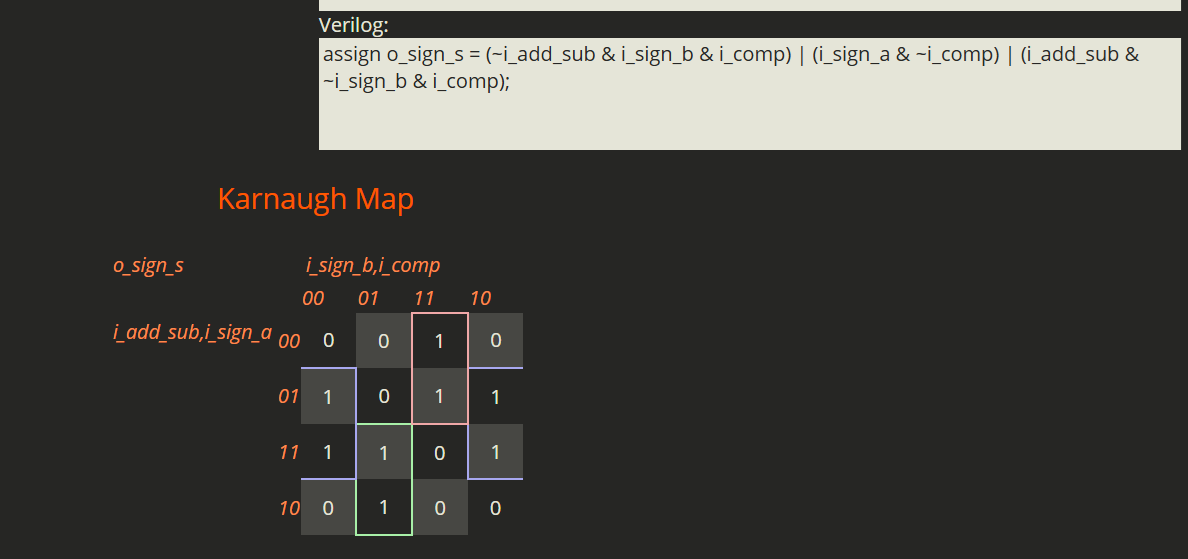
\includegraphics[width=.7\linewidth]{./my-chapters/my-images/K_maps/SIgn_unit.png}
	\caption{Rút gọn bìa K theo bảng sự thật \ref{tab: truth table for sign_unit}.}
\end{figure}

\subsection{Bộ xử lý các trường hợp đặc biệt ở ngõ vào}

\begin{figure}[H]
	\centering
	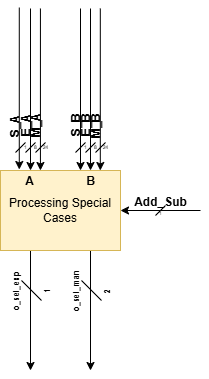
\includegraphics[width=.4\linewidth]{./my-chapters/my-diagrams/PSC.png}
\end{figure}
	
\begin{longtable}{|>{\centering\arraybackslash}m{3cm}
		|>{\centering\arraybackslash}m{4cm}
		|>{\centering\arraybackslash}m{4cm}
		|>{\centering\arraybackslash}m{4cm}|}
	\caption{Các giá trị đặc biệt ở ngõ vào.}
	
	\endfirsthead
	\multicolumn{3}{c}%
	{\tablename\ \thetable\ -- continued from previous page} \\ \hline
	\textsf{i\_add\_sub}	& \textsf{i\_data\_a} 	& \textsf{i\_data\_b} & \textsf{o\_data\_fpu} \\
	\endhead
	
	\hline \multicolumn{4}{r}{Continued on next page \dots} \\
	\endfoot
	
	\endlastfoot
		\hline
		\textsf{i\_add\_sub}	& \textsf{i\_data\_a} 	& \textsf{i\_data\_b} & \textsf{o\_data\_fpu} \\
%		\hline
%		0						& Number	 & $+ \infty$ & $+ \infty$ \\
%		\hline
%		0						& $+ \infty$ & Number	  & $+ \infty$ \\
%		\hline
%		0						& $+ \infty$ & $+ \infty$ & $+ \infty$ \\
%		\hline
%		0						& $+ \infty$ & $- \infty$ & $NaN$ \\
%		\hline
%		0						& $- \infty$ & $+ \infty$ & $NaN$ \\
%		\hline
%		0						& $- \infty$ & $- \infty$ & $- \infty$ \\
%		\hline
%		1						& $+ \infty$ & $+ \infty$ & $- \infty$ \\
%		\hline
%		1 						& $+ \infty$ & $- \infty$ & $NaN$ \\
%		\hline
%		1 						& $- \infty$ & $+ \infty$ & $- \infty$ \\
%		\hline
%		1 						& $- \infty$ & $- \infty$ & $NaN$ \\
%		\hline
%		0						& $NaN$		& X			  & $NaN$ \\
%		\hline
%		0						& X			&$NaN$		  & $NaN$ \\
%		\hline
%		1						& $NaN$		& X			  & $NaN$ \\
%		\hline
%		1						& X			& $NaN$		  & $NaN$ \\
%		\hline
		
		\hline
		0	& $+ \infty$ 	& Number 		& $+ \infty$ \\
		\hline 	
		0	& $+ \infty$ 	& $- \infty$ 	& NaN		 \\
		\hline
		0 	& $+ \infty$ 	& $+ \infty$ 	& $+ \infty$ \\
		\hline
		0 	& $- \infty$	& Number		& $- \infty$ \\
		\hline
		0	& $- \infty$	& $- \infty$	& $- \infty$ \\
		\hline
		0 	& $- \infty$ 	& $+ \infty$	& NaN		 \\
		\hline
		0 	& NaN			& X				& NaN		 \\
		\hline
		0 	& X				& NaN			& NaN		 \\
		\hline
		1	& $+ \infty$ 	& Number 		& $+ \infty$ \\
		\hline
		1	& Number 		& $+ \infty$ 	& $- \infty$ \\
		\hline 	
		1	& $+ \infty$ 	& $- \infty$ 	& $+ \infty$ \\
		\hline
		1 	& $+ \infty$ 	& $+ \infty$ 	& NaN	 	 \\
		\hline
		1 	& $- \infty$	& Number		& $- \infty$ \\
		\hline
		1 	&  Number		& $- \infty$	& $+ \infty$ \\
		\hline
		1	& $- \infty$	& $- \infty$	& NaN	 	 \\
		\hline
		1 	& $- \infty$ 	& $+ \infty$	& $- \infty$\\
		\hline
		1 	& NaN			& X				& NaN		 \\
		\hline
		1 	& X				& NaN			& NaN		 \\
		\hline
\end{longtable}

Với các giá trị đặc biệt ở ngõ vào có đặc tính đặc biệt như sau:

\begin{itemize}
	\item Đối với các số liên quan đến $\pm \infty$ thì có 
		\begin{itemize}
			\item Exponent: $E = 8'hFF$
			\item Mantissa: $M = 24'h00$
		\end{itemize}
	\item Đối với các số liên quan đến $NaN$ thì có 
	\begin{itemize}
		\item Exponent: $E = 8'hFF$
		\item Mantissa: $M \neq 24'h00$
	\end{itemize}
\end{itemize}

Từ đó ta tạo ra hai giá trị:

\begin{itemize}[label=+, leftmargin=2cm]
	\item \texttt{E} = $\& i\_Exponent$
	\item \texttt{M} = $\sim |(i\_Mantissa)$
\end{itemize}

\begin{longtable}{|>{\centering\arraybackslash}m{2cm}
		||>{\centering\arraybackslash}m{0.75cm}
		|>{\centering\arraybackslash}m{0.75cm}
		|>{\centering\arraybackslash}m{0.75cm}
		||>{\centering\arraybackslash}m{0.75cm}
		|>{\centering\arraybackslash}m{0.75cm}
		|>{\centering\arraybackslash}m{0.75cm}
		||>{\centering\arraybackslash}m{0.75cm}
		|>{\centering\arraybackslash}m{0.75cm}
		|>{\centering\arraybackslash}m{0.75cm}
		|>{\centering\arraybackslash}m{1.5cm}
		|>{\centering\arraybackslash}m{1.5cm}|}
	\caption{Bảng sự thật của bộ phát hiện các giá trị đặc biệt.}
	
	\endfirsthead
	\multicolumn{11}{c}{\tablename\ \thetable\ -- continued from previous page} \\ \hline
	\endhead
	
	\hline \multicolumn{11}{r}{Continued on next page \dots} \\
	\endfoot
	
	\endlastfoot
	\hline
	\multirow{2}{*}{\textsf{i\_add\_sub}} & \multicolumn{3}{c||}{\texttt{A}} & \multicolumn{3}{c||}{\texttt{B}} & \multicolumn{5}{c|}{\texttt{S}} \\
	\cline{2-12}
			& S	& E	& M	& S	& E	& M	& S	& E	& M	& S\_M\_1 & S\_M\_0\\
	\hline
	0		& 0 & 1 & 1 & X & 0 & X & 0 & 1 & 1 & 1 & 0 \\
	\hline
	0		& 0 & 1 & 1 & 1 & 1 & 1 & 0 & 1 & 0 & 1 & 1 \\
	\hline
	0 		& 0 & 1 & 1 & 0 & 1 & 1 & 0 & 1 & 1 & 1 & 0 \\
	\hline
	0		& 1 & 1 & 1 & X & 0 & X & 1 & 1 & 1 & 1 & 0 \\
	\hline
	0		& 1 & 1	& 1 & 1 & 1 & 1 & 1 & 1 & 1 & 1 & 0 \\
	\hline 
	0 		& 1 & 1 & 1 & 0 & 1 & 1 & 1 & 1 & 0 & 1 & 1 \\
	\hline
	0		& X & 1 & 0 & X & X & X & X & 1 & 0 & 1 & 1 \\
	\hline
	0		& X & X & X & X & 1 & 0 & X & 1 & 0 & 1 & 1 \\
	\hline
	1		& 0	& 1 & 1 & X & 0 & X & 0 & 1 & 1 & 1 & 0 \\
	\hline
	1 		& X & 0 & X & 0 & 1 & 1 & 1 & 1 & 1 & 1 & 0 \\
	\hline
	1		& 0 & 1 & 1 & 1 & 1 & 1 & 0 & 1 & 1 & 1 & 0 \\
	\hline
	1 		& 0 & 1 & 1 & 0 & 1 & 1 & X & 1 & 0 & 1 & 1 \\
	\hline
	1 		& 1 & 1 & 1 & X & 0 & X & 1 & 1 & 1 & 1 & 0 \\
	\hline
	1		& X & 0 & X & 1 & 1 & 1 & 0 & 1 & 1 & 1 & 0 \\
	\hline
	1		& 1 & 1 & 1 & 1 & 1 & 1 & X & 1 & 0 & 1 & 1 \\
	\hline
	1		& 1 & 1 & 1 & 0 & 1 & 1 & 1 & 1 & 1 & 1 & 0 \\
	\hline
	1 		& X & 1 & 0 & X & X & X & X & 1 & 0 & 1 & 1 \\
	\hline
	1		& X & X & X & X & 1 & 0 & X & 1 & 0 & 1 & 1 \\
	\hline
\end{longtable}

\subsection{Bộ căn chỉnh Exponent}

\begin{figure}[H]
	\centering
	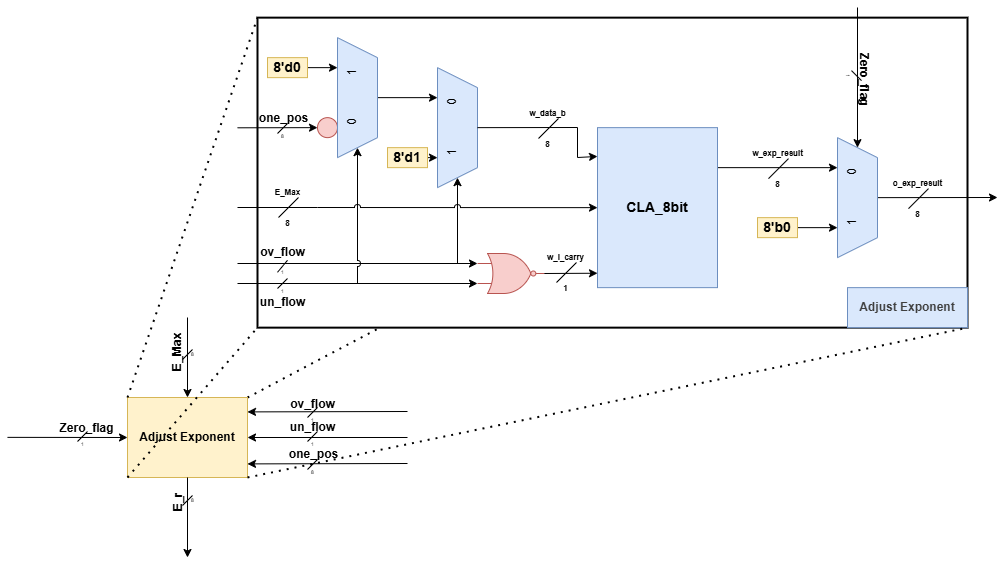
\includegraphics[width=\linewidth]{./my-chapters/my-diagrams/EXP_adjust.png}
\end{figure}

\subsection{Bộ cộng trừ Mantissa}

\begin{figure}[H]
\centering
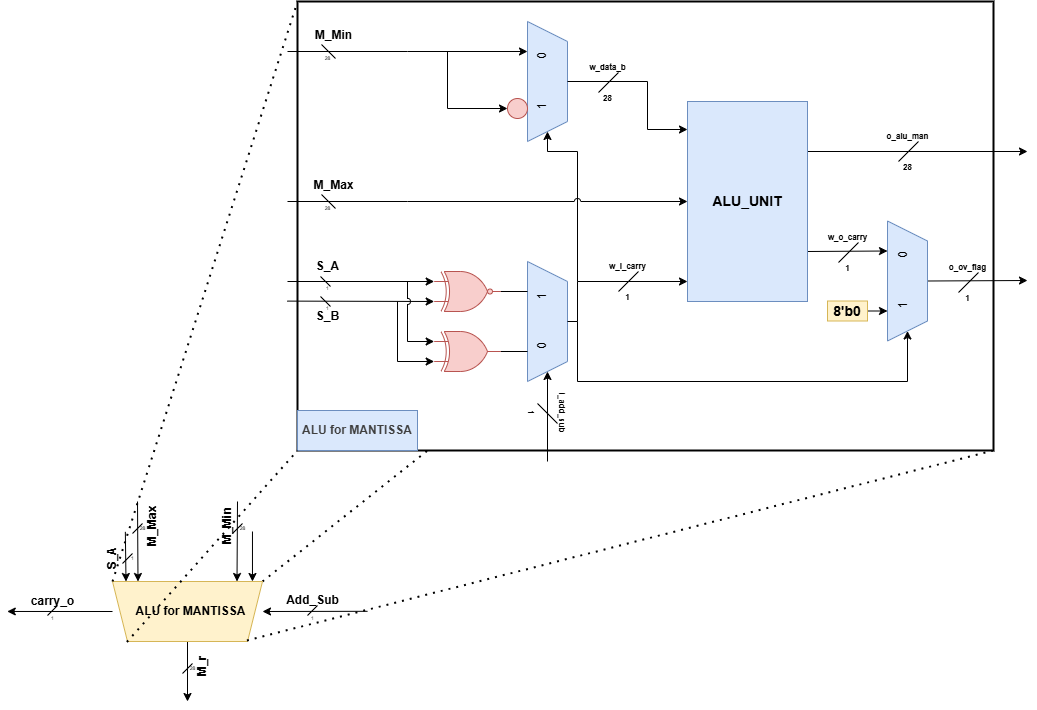
\includegraphics[width=\linewidth]{./my-chapters/my-diagrams/ALU_MAN.png}
\end{figure}

Tại bộ \textsf{ALU\_UNIT}, nhóm em sử dụng một bộ cộng với 28-bit

\begin{figure}[H]
	\centering
	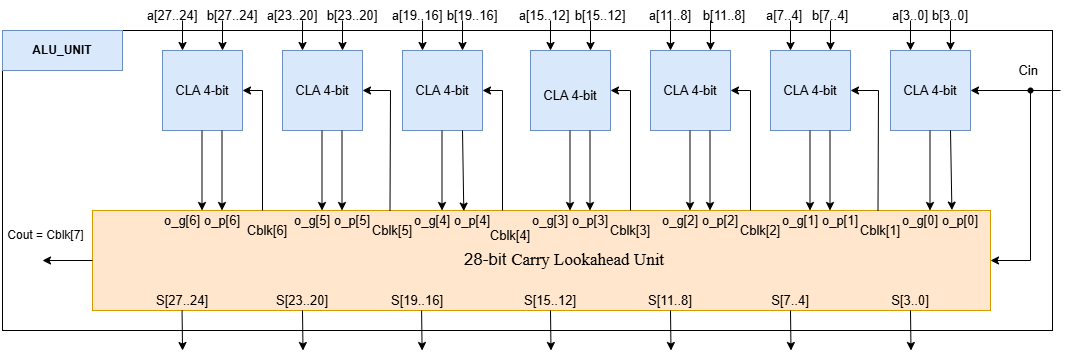
\includegraphics[width=.9\linewidth]{./my-chapters/my-diagrams/cla_28bit.png}
\end{figure} 

\subsection{Bộ chuẩn hóa Mantissa}

\begin{figure}[H]
	\centering
	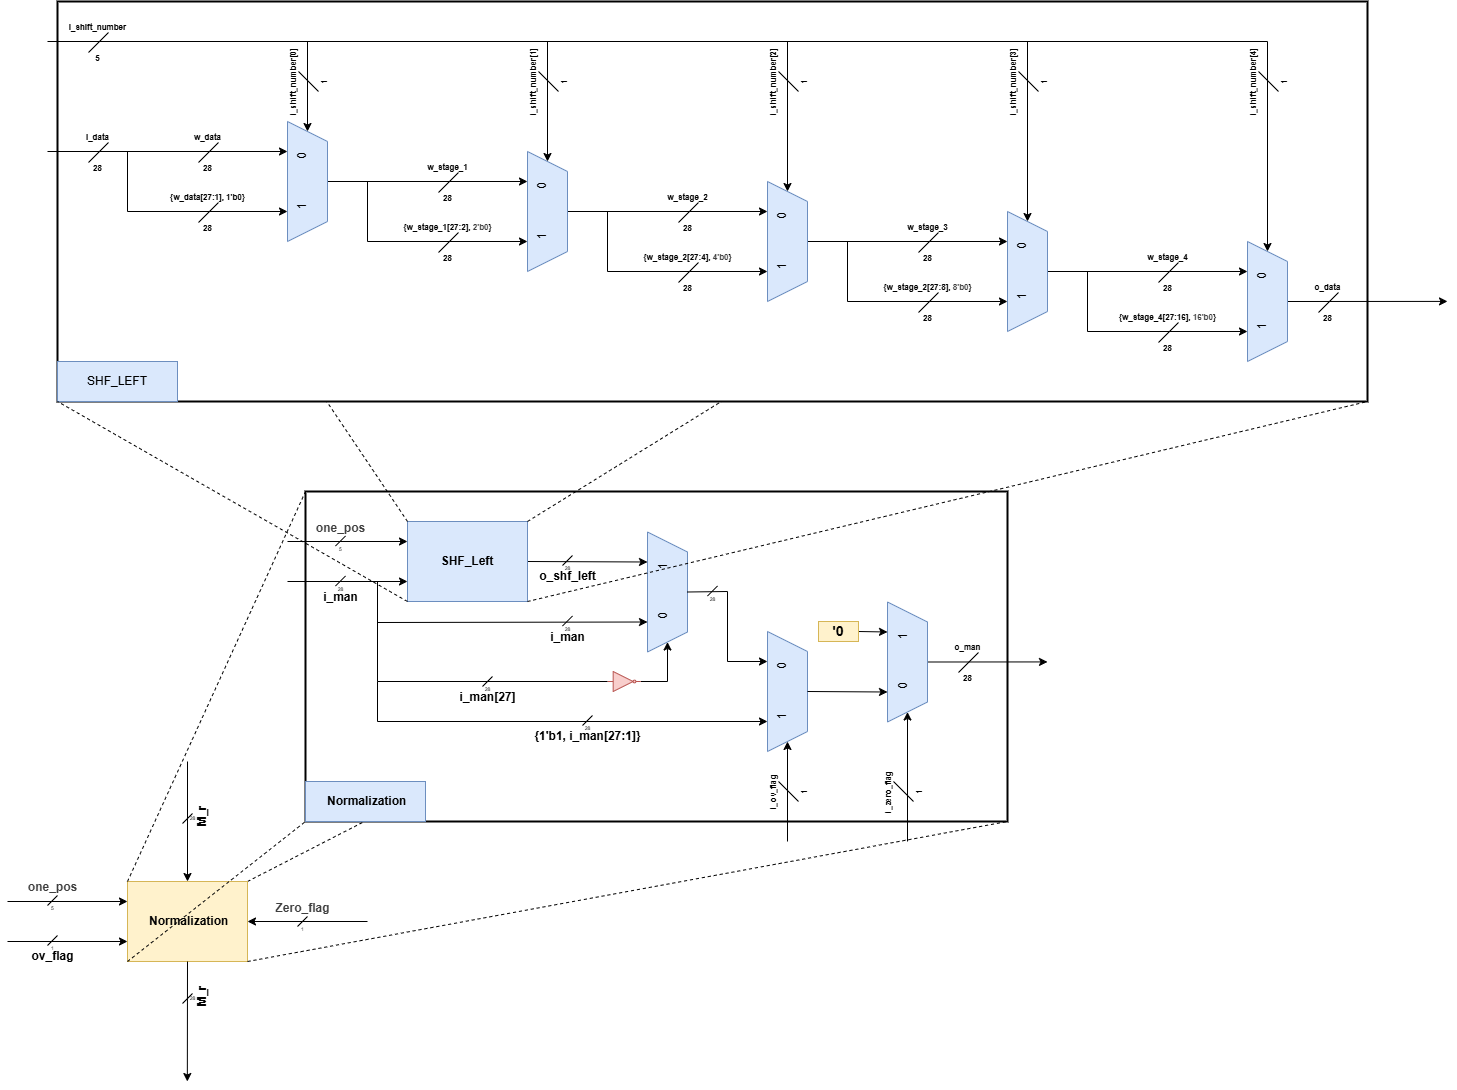
\includegraphics[width=\linewidth]{./my-chapters/my-diagrams/Normalization.png}
\end{figure}

\subsection{Bộ tìm vị trí bit 1 của MANTISSA sau khi chuẩn hóa}

\begin{figure}[H]
	\centering
	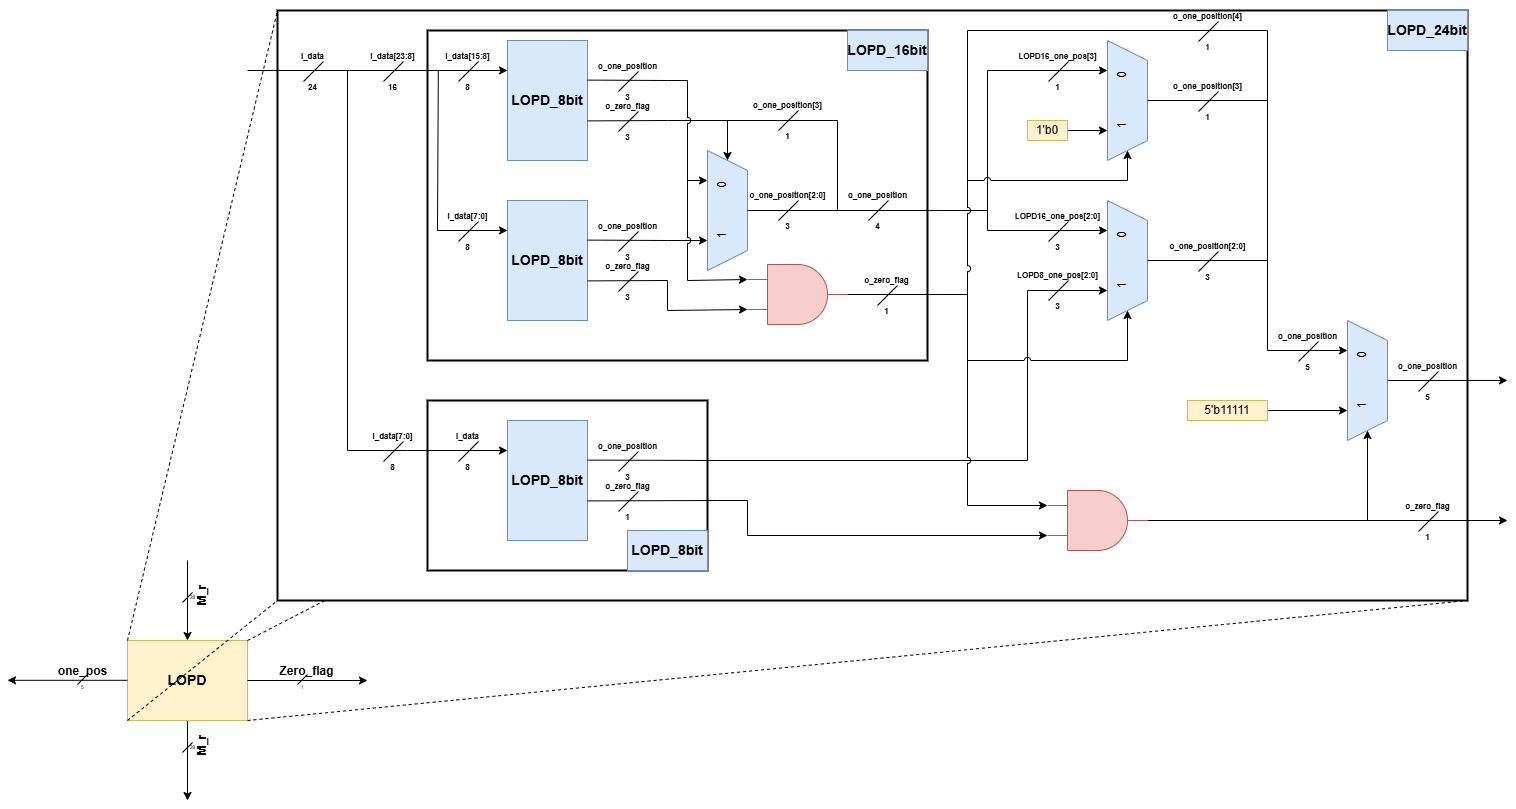
\includegraphics[width=\linewidth]{./my-chapters/my-diagrams/LODP_24bit.png}
\end{figure}

\subsection{Bộ làm tròn cho giá trị Mantissa và Exponent}

\begin{figure}[H]
	\centering
	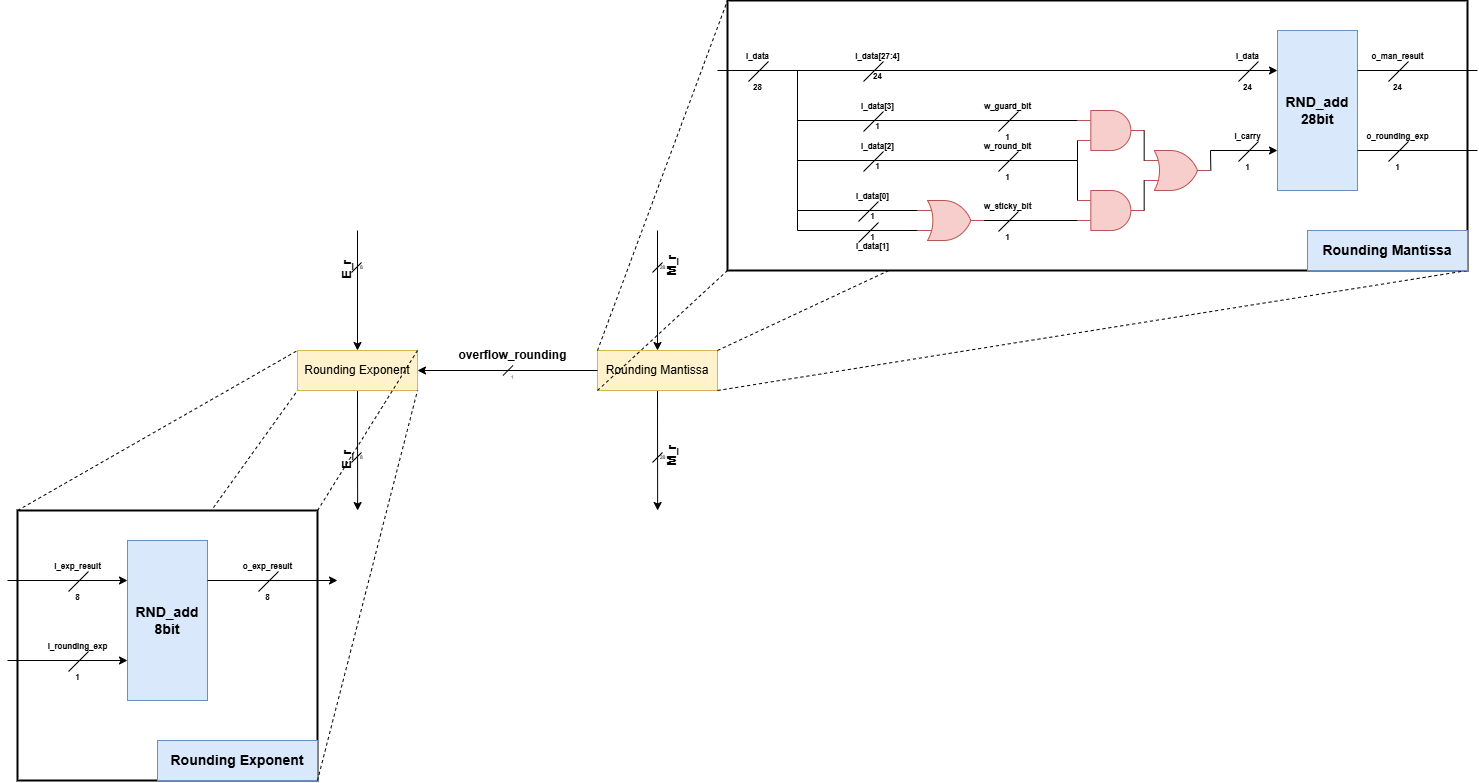
\includegraphics[width=\linewidth]{./my-chapters/my-diagrams/rounding.png}
\end{figure}

Ở đây bộ \texttt{RND\_unit} là bộ cộng giá trị làm tròn cho dữ liệu đầu vào, với kiểu làm tròn là làm tròn gần nhất. Vì vậy, ở đây ta thấy ở đây chỉ lấy \textsf{i\_data} + \textsf{i\_carry} bởi vì chỉ là cộng thêm 1 hoặc không. 

\begin{minipage}{.38\linewidth}
	\begin{lstlisting}[style=StyleCode, language=SystemVerilog, linewidth=.9\linewidth]
		p = a ^ b;
		g = a & b;
		c[i] = g[i] | (p[i] & c[i-1])
	\end{lstlisting}
\end{minipage}
\begin{minipage}{.1\linewidth}
	\hspace{0.5cm}
	$\Rightarrow$
\end{minipage}
\begin{minipage}{.38\linewidth}
	\begin{lstlisting}[style=StyleCode, language=SystemVerilog, linewidth=.9\linewidth]
		p = a;
		c[i] = g[i] | (p[i] & c[i-1])
		
		s 	= p ^ c
		c_o	= &a & c[0]
	\end{lstlisting}
\end{minipage}
